\documentclass[a4paper,12pt]{article}
\usepackage[UTF8]{ctex}
\usepackage{amsmath,amsthm,amssymb}
\usepackage{graphicx}
\usepackage{geometry}
\usepackage{array}
\usepackage{pgfplots}
\usepackage{pgfplotstable}
\usepackage{tikz}
\usepackage{multirow}
\usepackage{enumitem}
\pgfplotsset{compat=1.18}
\geometry{left=2cm, right=2cm, top=2cm, bottom=2cm}

\title{复变函数期中复习}
\author{核31\kern 36pt 钱昊远\kern 12pt 整理}
\date{2024年11月2日}

\begin{document}

\maketitle

\section{复数}

\subsection{复数的表示与运算}

\noindent
\textbf{复数的表示}

$$
z=x+yi=r(\cos\theta+i\sin\theta)=re^{i\theta}
$$

其中$r=\left|z\right|=\sqrt{x^2+y^2}$为复数$z$的模,$\theta=\text{Arg}\ z$为复数$z$的辐角,
用$\arg z$表示$z$的主辐角($-\pi<\arg z\le\pi$),$\text{Arg}\ z=\arg z+2k\pi(k\in\mathbb Z)$。

\noindent
\textbf{棣莫弗(De Moivre)公式}

$$
(\cos\theta+i\sin\theta)^n=\cos n\theta+i\sin n\theta
$$

\noindent
\textbf{$n$次方根}

若$w^n=z$,则
$$
w=\left|z\right|^{\frac1n}\left\{\cos\left[\frac1n\left(\arg z+2k\pi\right)\right]
+i\sin\left[\frac1n\left(\arg z+2k\pi\right)\right]\right\}
$$
其中$k=0,1,\dots,n-1$。

\subsection{平面点集与平面曲线}

\noindent
\textbf{邻域}

\noindent
\textbf{平面点集的类型}

\noindent
\textbf{区域与闭区域}

\noindent
\textbf{简单闭曲线}

\subsection{无穷大与复球面}

\noindent
\textbf{无穷大}

可以定义一个特殊的复数——无穷大:
$$
\infty=\frac10
$$

\noindent
\textbf{扩充复平面}

可设想复平面上有一理想点与$\infty$相对应,此点称为无穷远点,复平面加上无穷远点称为扩充复平面。
即$\overline{\mathbb{C}}=\mathbb{C}\cup\left\{\infty\right\}$。

\noindent
\textbf{复球面}

\begin{center}
    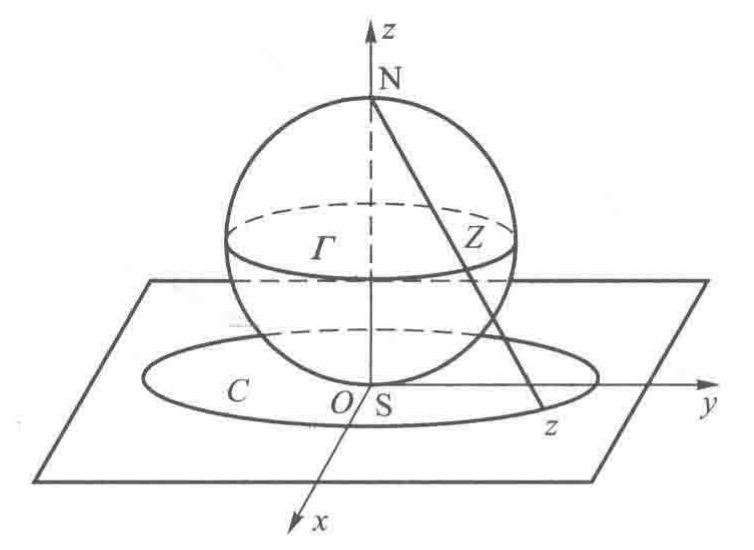
\includegraphics[width=10cm]{复球面.png}
\end{center}

\section{复变函数}

\subsection{基本知识}

\noindent
\textbf{定义、单值函数、多值函数}

\noindent
\textbf{像与原像(参见课本第六章)}

\noindent
\textbf{极限、连续性}

\subsection{解析函数}

\noindent
\textbf{导数与微分}

设函数$w=f\left(z\right)$在点$z_0$的某邻域内有定义,$z_0+\Delta z$是邻域内任一点,若
$$
\lim_{\Delta z\to0}\frac{f\left(z_0+\Delta z\right)-f\left(z_0\right)}{\Delta z}
$$
存在有限的极限值$A$,则称$f\left(z\right)$在$z_0$处可导,记作
$$
f'\left(z_0\right)=\left.\frac{dw}{dz}\right|_{z=z_0}=
\lim_{\Delta z\to0}\frac{f\left(z_0+\Delta z\right)-f\left(z_0\right)}{\Delta z}=A
$$
也称
$$
df\left(z_0\right)=f'\left(z_0\right)dz
$$
为$f\left(z\right)$在$z_0$处的微分,故也称$f\left(z\right)$在$z_0$点可微。

\noindent
\textbf{解析}

若$f\left(z\right)$在$z_0$及$z_0$的邻域内处处可导,则称$f\left(z\right)$在$z_0$处解析;
若$f\left(z\right)$在区域$D$内每一点都解析,则称$f\left(z\right)$在$D$内解析,
或者说$f\left(z\right)$是$D$内的解析函数。
若$f\left(z\right)$在$z_0$处不解析,则称$z_0$为$f\left(z\right)$的奇点。

\begin{center}
    $f\left(z\right)$在$z_0$处解析$\Longrightarrow$$f\left(z\right)$在$z_0$处可导

    $f\left(z\right)$在区域$D$内解析$\Longleftrightarrow$$f\left(z\right)$在区域$D$内处处可导
\end{center}

解析函数求导的四则运算法则与链式法则略,反函数的求导法则如下:
设函数$w=f\left(z\right)$在区域$D$内解析且$f'\left(z\right)\ne0$,
又反函数$z=f^{-1}\left(w\right)=\varphi\left(w\right)$存在且连续,则
$$
\varphi'\left(w\right)=\left.\frac1{f'\left(z\right)}\right|_{z=\varphi\left(w\right)}
=\frac1{f'\left(\varphi\left(w\right)\right)}
$$

\noindent
\textbf{C-R方程}

函数$f\left(z\right)=u\left(x,y\right)+iv\left(x,y\right)$在$z=x+iy$处可导的充要条件是:
$u\left(x,y\right)$、$v\left(x,y\right)$在点$\left(x,y\right)$处可微,
而且满足柯西——黎曼方程:
$$
\frac{\partial u}{\partial x}=\frac{\partial v}{\partial y}\kern 36pt
\frac{\partial u}{\partial y}=-\frac{\partial v}{\partial x}
$$

在此条件下:
$$
f'\left(z\right)=\frac{\partial u}{\partial x}+i\frac{\partial v}{\partial x}
=\frac{\partial v}{\partial y}+i\frac{\partial v}{\partial x}
=\frac{\partial u}{\partial x}-i\frac{\partial u}{\partial y}
=\frac{\partial v}{\partial y}-i\frac{\partial u}{\partial v}
$$
也可记忆为:
$$
f'\left(z\right)=\frac{\partial f}{\partial x}=\frac1i\frac{\partial f}{\partial y}
$$

\noindent
\textbf{调和函数}

若二元实函数$\varphi\left(x,y\right)$在区域$D$内有二阶连续偏导数,且满足二维Laplace方程
$$
\frac{\partial^2\varphi}{\partial x^2}+\frac{\partial^2\varphi}{\partial y^2}=0
$$
则称$\varphi\left(x,y\right)$为区域$D$内的调和函数,
或说函数$\varphi\left(x,y\right)$在区域$D$内调和。

设函数$f\left(z\right)=u\left(x,y\right)+iv\left(x,y\right)$在区域$D$内解析,
则$f\left(z\right)$的实部$u\left(x,y\right)$和虚部$v\left(x,y\right)$都是
区域$D$内的调和函数。

设函数$\varphi\left(x,y\right)$及$\psi\left(x,y\right)$均为区域$D$内的调和函数,
且满足C-R方程
$$
\frac{\partial\varphi}{\partial x}=\frac{\partial\psi}{\partial y}\kern 36pt
\frac{\partial\varphi}{\partial y}=-\frac{\partial\psi}{\partial x}
$$
则称$\psi$是$\varphi$的共轭调和函数。($-\varphi$是$\psi$的共轭调和函数)

复变函数$f\left(z\right)=u\left(x,y\right)+iv\left(x,y\right)$在区域$D$内解析的充要条件是
在区域$D$内,$f\left(z\right)$的虚部$v\left(x,y\right)$是实部$u\left(x,y\right)$的共轭调和函数。

\subsection{初等函数}

\noindent
\textbf{指数函数}

$$
w=e^z=e^{x+iy}=e^x\left(\cos y+i\sin y\right)
$$

指数函数$f\left(z\right)=e^z$有如下性质:

指数函数是单值函数。

指数的运算法则(与实数的相同):
$$
e^{z_1}e^{z_2}=e^{z_1+z_2}
$$

$e^z$在全平面解析,且
$$
\left(e^z\right)'=e^z
$$

由$e^z=e^{x+iy}=e^xe^{iy}$可知
$$
\left|e^z\right|=e^x,\kern 12pt
\text{Arg}\ e^z=y+2k\pi(k\in\mathbb{Z})
$$
故$\forall z\in\mathbb{C}$,都有$e^z\ne0$。
又可得$e^z$是以$2k\pi i(k\in\mathbb{Z},k\ne0)$为周期的函数。

$e^z$当$z$趋于$\infty$时没有极限。

\noindent
\textbf{对数函数}

满足方程$e^w=z\left(z\ne0\right)$的函数$w=f\left(z\right)$称为对数函数,
$$
w=\text{Ln}\ z=\ln\left|z\right|+i\text{Arg}\ z\kern 12pt \left(z\ne0\right)
$$

对数函数$f\left(z\right)=\text{Ln}\ z$有如下性质:

因为$\text{Arg}\ z$是多值函数,故对数函数是多值函数,且每两个值相差$2k\pi$的整数倍。
如果规定$\text{Arg}\ z$取主值$\arg z$,就得到$\text{Ln}\ z$的一个单值“分支”,记作
$$
\ln z=\ln\left|z\right|+i\arg z
$$
并把它称为$\text{Ln}\ z$的主值。而其余各个值可由
$$
\text{Ln}\ z=\ln z+2k\pi i\kern 12pt \left(k\in\mathbb{Z},k\ne0\right)
$$
表达,对于每一个固定的$k$,上式为一单值函数,称为$\text{Ln}\ z$的一个分支。

对数的运算法则:(注意是$\text{Ln}$而不是$\ln$)
$$
\text{Ln}\left(z_1z_2\right)=\text{Ln}\ z_1+\text{Ln}\ z_2
$$
$$
\text{Ln}\frac{z_1}{z_2}=\text{Ln}\ z_1-\text{Ln}\ z_2
$$
注意:$\text{Ln}\ z^n=n\text{Ln}\ z\left(n\in\mathbb{N}_+,n>1\right)$不再成立。
这本质上是因为$\sum_{i=1}^n\text{Ln}\ z=n\text{Ln}\ z$不成立,
前者的两个相邻分支相差$2\pi i$,后者的两个相邻分支相差$2n\pi i$。

$\ln z$在除去原点及负实轴的复平面上解析,且
$$
\left(\ln z\right)'=\frac1z
$$
$\text{Ln}\ z$的各分支在除去原点及负实轴的复平面上也解析,且有相同的导数值。
(若更改$\arg z$的定义,可以改变$\text{Ln}\ z$的解析范围。)

\noindent
\textbf{幂函数}

函数$w=z^\alpha$规定为
$$
z^\alpha=e^{\alpha\text{Ln}\ z}\kern 12pt\left(\alpha\in\mathbb{C},z\ne0\right)
$$
当$\alpha$为正实数且$z=0$时,规定$z^\alpha=0$

幂函数在不同的$\alpha$值的情况下取值有所差异,详见课本。

$w=z^\alpha$(的相应分支)在除原点和负实轴的复平面内是解析的,
$$
\left(z^\alpha\right)'=\alpha z^{\alpha-1}
$$

\noindent
\textbf{三角函数}

$$
\cos z=\frac12\left(e^{iz}+e^{-iz}\right)
$$
$$
\sin z=\frac1{2i}\left(e^{iz}-e^{-iz}\right)
$$
注:当$z$为实数时,该定义与实数范围内的三角函数定义等价。
其余的三角函数可由$\cos z$与$\sin z$导出,此处不再列出。

余弦函数$\cos z$和正弦函数$\sin z$的性质如下:

正余弦函数的许多性质(单值性、周期性、奇偶性、运算法则)与实数范围内的相同。
特别的,$\left|\sin z\right|\le1$与$\left|\cos z\right|\le1$在复数范围内不再成立,
且$\sin z$与$\cos z$都是无界的。

正余弦函数在复平面上解析,
$$
\left(\cos z\right)'=-\left(\sin z\right)\kern 36pt
\left(\sin z\right)'=\left(\cos z\right)
$$

\noindent
\textbf{反三角函数}

\noindent
\textbf{双曲函数与反双曲函数}

\section{级数}

\subsection{复数项级数与复变函数项级数}

\noindent
\textbf{复数项级数}

设$\left\{z_n\right\}\left(n=1,2,\cdots\right)$为一复数序列,表达式
$$
\sum_{n=1}^\infty z_n=z_1+z_2+\cdots+z_n+\cdots
$$
称为复数项无穷级数。若它的部分和序列
$$
S_n=\sum_{k=1}^n z_k=z_1+z_2+\cdots+z_n
$$
有极限$\lim_{n\to\infty}S_n=S$($S$为有限复数),则称级数是收敛的,$S$称为级数的和;
若不然,则称级数是发散的。

复数项级数的部分和序列
$$
S_n=\sum_{k=1}^n z_k=\sum_{k=1}^n x_k+i\sum_{k=1}^n y_k
$$
易知级数$\sum_{n=1}^\infty z_n$收敛当且仅当
$\sum_{n=1}^\infty x_n$与$\sum_{n=1}^\infty y_n$都收敛。

级数$\sum_{n=1}^\infty z_n$收敛的必要条件为
$$
\lim_{n\to\infty}z_n=\lim_{n\to\infty}\left(x_n+iy_n\right)=0
$$

如果级数$\sum_{n=1}^\infty \left|z_n\right|$收敛,则级数$\sum_{n=1}^\infty z_n$收敛,
此时称级数$\sum_{n=1}^\infty z_n$绝对收敛。
如果$\sum_{n=1}^\infty z_n$收敛而$\sum_{n=1}^\infty \left|z_n\right|$不收敛,
称$\sum_{n=1}^\infty z_n$条件收敛。

\noindent
\textbf{复变函数项级数}

设$\left\{f_n\left(z\right)\right\}$为区域$D$内的函数,则称
$$
\sum_{n=1}^\infty f_n\left(z\right)=f_1\left(z\right)+f_2\left(z\right)+\cdots+f_n\left(z\right)+\cdots
$$
为区域$D$内的复变函数项级数。该级数的前$n$项和
$$
S_n\left(z\right)=\sum_{k=1}^n f_k\left(z\right)=f_1\left(z\right)+f_2\left(z\right)+\cdots+f_n\left(z\right)
$$
称为级数的部分和。

设$z_0$为区域$D$内的一点,若$\lim_{n\to\infty}S_n\left(z_0\right)=S\left(z_0\right)$存在,
则称级数$\sum_{n=1}^\infty f_n\left(z\right)$在$z_0$处是收敛的,
此时$S\left(z_0\right)$就是它的和,即$\sum_{n=1}^\infty f_n\left(z_0\right)=S\left(z_0\right)$。
若级数在$D$内处处收敛,则级数的和就是$D$内的一个函数$S\left(z\right)$,即
$$
\sum_{n=1}^\infty f_n\left(z\right)=S\left(z\right)
$$

\subsection{幂级数}

\noindent
\textbf{幂级数定义}

形如
$$
\sum_{n=0}^\infty C_n\left(z-z_0\right)^n
=C_0+C_1\left(z-z_0\right)+C_2\left(z-z_0\right)^2+\cdots+C_n\left(z-z_0\right)^n+\cdots
$$
的复变函数项级数称为幂级数。其中$C_n\left(n=0,1,2,\cdots\right)$与$z_0$均为复常数。

\noindent
\textbf{阿贝尔定理}

若幂级数在点$z_1\left(z_1\ne z_0\right)$处收敛,则级数在圆域
$\left|z-z_0\right|<\left|z_1-z_0\right|$内绝对收敛。

若幂级数在点$z_2\left(z_2\ne z_0\right)$处发散,则满足
$\left|z-z_0\right|>\left|z_2-z_0\right|$的点$z$使级数发散。

\noindent
\textbf{收敛半径}

若存在一个有限正数$R$,使得$\sum_{n=0}^\infty C_n\left(z-z_0\right)^n$
在圆周$\left|z-z_0\right|=R$内绝对收敛,在圆周$\left|z-z_0\right|=R$的外部发散,
则$R$称为此幂级数的收敛半径。
特别的,若对任意的$z\ne z_0$,级数$\sum_{n=0}^\infty C_n\left(z-z_0\right)^n$均发散,则$R=0$;
若对任意的$z$,级数$\sum_{n=0}^\infty C_n\left(z-z_0\right)^n$均收敛,则$R=\infty$。

比值法:若
$$
\lim_{n\to\infty}\left|\frac{C_{n+1}}{C_n}\right|=\lambda
$$
则幂级数的收敛半径$R=\frac1\lambda$;

根值法:若
$$
\lim_{n\to\infty}\sqrt[n]{\left|C_n\right|}=\lambda
$$
则幂级数的收敛半径$R=\frac1\lambda$。

\noindent
\textbf{运算法则}

同实变量幂级数一样,复变量幂级数也能进行加、减、乘、代换等运算,
且在收敛圆内部,幂级数的和是一个解析函数,可以逐项求导及逐项积分任意次。

\subsection{泰勒级数}

\noindent
\textbf{泰勒定理}

设函数$f\left(z\right)$在区域$D$内解析,$z_0$为$D$内的一点,$R$为$z_0$到$D$的边界上各点的最短距离,
则当$\left|z-z_0\right|<R$时,$f\left(z\right)$可展为幂级数
$$
f\left(z\right)=\sum_{n=0}^\infty C_n\left(z-z_0\right)^n
$$
其中$C_n=\frac1{n!}f^{(n)}\left(z_0\right),\kern 12pt n=0,1,2,\cdots$

函数在一点解析的充要条件是它在这点的邻域内可以展开为幂级数。

\noindent
\textbf{常见的泰勒级数}

$$
\frac1{1-z}=\sum_{n=0}^\infty z^n
=1+z+z^2+\cdots+z^n+\cdots
$$
上述级数收敛域为$\left|z\right|<1$,下列级数收敛域为$\left|z\right|<+\infty$

$$
e^z=\sum_{n=0}^\infty \frac1{n!}z^n
=1+\frac{z}{1!}+\frac{z^2}{2!}+\cdots+\frac{z^n}{n!}+\cdots
$$

$$
\sin z=\sum_{n=0}^\infty \left(-1\right)^n\frac{z^{2n+1}}{\left(2n+1\right)!}
=z-\frac{z^3}{3!}+\frac{z^5}{5!}+\cdots+
\left(-1\right)^n\frac{z^{2n+1}}{\left(2n+1\right)!}+\cdots
$$

$$
\cos z=\sum_{n=0}^\infty \left(-1\right)^n\frac{z^{2n}}{\left(2n\right)!}
=1-\frac{z^2}{2!}+\frac{z^4}{4!}+\cdots+
\left(-1\right)^n\frac{z^{2n}}{\left(2n\right)!}+\cdots
$$

$$
\left(1+z\right)^\alpha=1+\sum_{n=1}^\infty\frac{\prod_{k=0}^{n-1}\left(\alpha-k\right)}{n!}z^n
=1+\alpha z+\frac{\alpha\left(\alpha-1\right)}{2!}z^2+\cdots+
\frac{\alpha\left(\alpha-1\right)\cdots\left(\alpha-n+1\right)}{n!}z^n+\cdots
$$

\subsection{洛朗级数}

\noindent
\textbf{洛朗定理}

设函数$f\left(z\right)$在圆环域$R_1<\left|z-z_0\right|<R_2$内处处解析,
则$f\left(z\right)$一定能在此圆环域中展开为
$$
f\left(z\right)=\sum_{n=-\infty}^\infty C_n\left(z-z_0\right)^n
$$
其中
$$
C_n=\frac1{2\pi i}\oint_C\frac{f\left(\zeta\right)}{\left(\zeta-z_0\right)^{n+1}}d\zeta
\kern 12pt\left(n\in\mathbb{Z}\right)
$$
而$C$为此圆环域内绕$z_0$的任一简单闭曲线。
注意:不能将$C_n$写成$\frac{f^{\left(n\right)}\left(z_0\right)}{n!}$,
因为$f\left(z\right)$在$\left|z-z_0\right|\le R_1$内不一定处处解析。

洛朗级数中的正整次幂部分称为解析部分,其在$\left|z-z_0\right|<R_2$内收敛;
负整次幂部分称为主要部分,其在$\left|z-z_0\right|>R_1$内收敛。

\noindent
\textbf{洛朗级数的展开方法}

洛朗级数的展开,一般采用在已知泰勒级数的收敛域内使用泰勒展开的方式展开。常见的方式为:
在$\left|z-z_0\right|<R_2$内展开
$$
\left(z-z_0\right)^k\frac1{1-\left(\frac{z-z_0}{r}\right)^l}=
\sum_{n=0}^\infty \frac1{r^{ln}}\left(z-z_0\right)^{ln+k}
$$
其中$r\ge R_2,k\in\mathbb{Z},l\in\mathbb{N}_+$;
或在$\left|z-z_0\right|>R_1$内展开
$$
\left(z-z_0\right)^k\frac1{1-\left(\frac{r}{z-z_0}\right)^l}=
\sum_{n=0}^\infty r^{ln}\frac1{\left(z-z_0\right)^{ln-k}}
$$
其中$0<r\le R_1,k\in\mathbb{Z},l\in\mathbb{N}_+$。

\section{留数}

\subsection{孤立奇点与零点}

\noindent
\textbf{有限孤立奇点的定义}

若$f\left(z\right)$在$z_0$处不解析,但在$z_0$的某一个去心邻域$0<\left|z-z_0\right|<\delta$内处处解析,
则称$z_0$为$f\left(z\right)$的孤立奇点。

在孤立奇点$z=z_0$的去心邻域内,函数$f\left(z\right)$可展开为洛朗级数
$$
f\left(z\right)=\sum_{n=-\infty}^\infty C_n\left(z-z_0\right)^n
$$
函数在$z_0$处的奇异性质完全体现在洛朗级数的负整次幂部分,即主要部分。

\noindent
\textbf{有限孤立奇点的分类}

若对一切$n<0$有$C_n=0$,则称$z_0$是函数$f\left(z\right)$的可去奇点。
此时若令$f\left(z_0\right)=C_0$,可以得到在整个圆盘$\left|z-z_0\right|<\delta$内解析的函数$f\left(z\right)$。

若只有有限个(至少一个)整数$n<0$,使得$C_n\ne0$,则称$z_0$是函数$f\left(z\right)$的极点。
设对于正整数$m$,$C_{-m}\ne0$,而当$n<-m$时,$C_n=0$,则称$z_0$是函数$f\left(z\right)$的$m$阶极点,
$1$阶极点又叫做简单极点。

若有无限个整数$n<0$,使得$C_n\ne0$,则称$z_0$是函数$f\left(z\right)$的本性奇点。

当函数$f\left(z\right)$在$0<\left|z-z_0\right|<\delta\left(0<\delta\le+\infty\right)$内解析时:
\begin{center}
    $\lim_{z\to z_0}f\left(z\right)=C_0\ne\infty$
    $\Longleftrightarrow$
    $z_0$是$f\left(z\right)$的可去奇点

    $\lim_{z\to z_0}f\left(z\right)=\infty$
    $\Longleftrightarrow$
    $z_0$是$f\left(z\right)$的极点

    $\lim_{z\to z_0}\left(z-z_0\right)^mf\left(z\right)=C_{-m}\ne0\left(m\in\mathbb{N}_+\right)$
    $\Longleftrightarrow$
    $z_0$是$f\left(z\right)$的$m$阶极点

    $\lim_{z\to z_0}f\left(z\right)$不存在
    $\Longleftrightarrow$
    $z_0$是$f\left(z\right)$的本性奇点
\end{center}

\noindent
\textbf{有限极点与零点的关系}

若$f\left(z\right)=\left(z-z_0\right)^m\varphi\left(z\right)\kern 12pt\left(m\in\mathbb{N}_+\right)$,
$\varphi\left(z\right)$在$z_0$处解析,且$\varphi\left(z_0\right)\ne0$,
则称$z_0$为$f\left(z\right)$的$m$阶零点。一个不恒为零的解析函数的零点是孤立的。

若$f\left(z_0\right)$在$z_0$解析,那么$z_0$为$f\left(z\right)$的$m$阶零点的充要条件为
$$
f^{\left(n\right)}\left(z_0\right)=0\kern 12pt
\left(n=0,1,\cdots,m-1\right),\kern 12pt
f^{\left(m\right)}\left(z_0\right)\ne0
$$

函数的零点与极点的关系为(可去奇点当做解析点看待):
\begin{center}
    $z_0$是$f\left(z\right)$的$m$阶极点
    $\Longleftrightarrow$
    $z_0$是$\frac1{f\left(z\right)}$的$m$阶零点
\end{center}

\noindent
\textbf{无穷远点}

设函数$f\left(z\right)$在无穷远点的邻域$R<\left|z\right|<+\infty$内解析,
则无穷远点$\infty$称为$f\left(z\right)$的孤立奇点。

在$R<\left|z\right|<+\infty$内,$f\left(z\right)$有洛朗级数展开式
$$
f\left(z\right)=\sum_{n=-\infty}^\infty C_nz^n
=\sum_{n=-\infty}^\infty \frac{C_{-n}}{z^n}
\kern 12pt\left(R<\left|z\right|<+\infty\right)
$$
其中$\sum_{n=-\infty}^0 C_nz^n$为解析部分,$\sum_{n=1}^\infty C_nz^n$为主要部分。

若对一切$n>0$有$C_n=0$,则称$\infty$是函数$f\left(z\right)$的可去奇点。

若只有有限个(至少一个)整数$n>0$,使得$C_n\ne0$,则称$\infty$是函数$f\left(z\right)$的极点。
设对于正整数$m$,$C_m\ne0$,而当$n>m$时,$C_n=0$,则称$\infty$是函数$f\left(z\right)$的$m$阶极点。

若有无限个整数$n>0$,使得$C_n\ne0$,则称$\infty$是函数$f\left(z\right)$的本性奇点。

当函数$f\left(z\right)$在$R<\left|z\right|<-\infty\left(R\ge0\right)$内解析时:
\begin{center}
    $\lim_{z\to\infty}f\left(z\right)=C_0\ne\infty$
    $\Longleftrightarrow$
    $\infty$是$f\left(z\right)$的可去奇点

    $\lim_{z\to\infty}f\left(z\right)=\infty$
    $\Longleftrightarrow$
    $\infty$是$f\left(z\right)$的极点

    $\lim_{z\to\infty}\frac{f\left(z\right)}{z^m}=C_{m}\ne0\left(m\in\mathbb{N}_+\right)$
    $\Longleftrightarrow$
    $\infty$是$f\left(z\right)$的$m$阶极点

    $\lim_{z\to\infty}f\left(z\right)$不存在
    $\Longleftrightarrow$
    $\infty$是$f\left(z\right)$的本性奇点
\end{center}

\subsection{留数的定义与计算}

\noindent
\textbf{有限孤立奇点处留数的定义}

设$z_0$是解析函数$f\left(z\right)$的有限孤立奇点,把$f\left(z\right)$在$z_0$处的洛朗展开式中
的负一次幂的系数$C_{-1}$称为$f\left(z\right)$在$z_0$处的留数,记作
$$
\text{Res}\left[f\left(z\right),z_0\right]=C_{-1}
$$
易知若$z_0$为$f\left(z\right)$的有限可去奇点,则$\text{Res}\left[f\left(z\right),z_0\right]=0$。

\noindent
\textbf{函数在有限极点的留数}

若$z_0$为$f\left(z\right)$的$m\left(m\in\mathbb{N}_+\right)$阶极点,则
$$
\text{Res}\left[f\left(z\right),z_0\right]=\frac1{\left(m-1\right)!}
\lim_{z\to z_0}\frac{d^{m-1}}{dz^{m-1}}\left[\left(z-z_0\right)^mf\left(z\right)\right]
$$
其中当$m=1$时,即$z_0$为简单极点时,
$$
\text{Res}\left[f\left(z\right),z_0\right]=
\lim_{z\to z_0}\left[\left(z-z_0\right)f\left(z\right)\right]
$$

设$f\left(z\right)=\frac{P\left(z\right)}{Q\left(z\right)}$,
其中$P\left(z\right)$与$Q\left(z\right)$均在$z_0$处解析,
若$P\left(z_0\right)\ne0$,$z_0$为$Q\left(z\right)$的一阶零点,
则$z_0$为$f\left(z\right)$的一阶极点,且
$$
\text{Res}\left[f\left(z\right),z_0\right]=\frac{P\left(z_0\right)}{Q'\left(z_0\right)}
$$

\noindent
\textbf{函数在无穷远点的留数}

设$\infty$为$f\left(z\right)$的一个孤立奇点,把$f\left(z\right)$在$R<\left|z\right|<+\infty$
内的洛朗展开式中的负一次幂的系数的相反数$-C_{-1}$称为$f\left(z\right)$在$\infty$处的留数,记作
$$
\text{Res}\left[f\left(z\right),\infty\right]=-C_{-1}
$$
注意:即使$\infty$为$f\left(z\right)$的可去奇点,$\text{Res}\left[f\left(z\right),\infty\right]$也未必是$0$。

无穷远点的留数可以转化为坐标原点的留数:
$$
\text{Res}\left[f\left(z\right),\infty\right]=
-\text{Res}\left[f\left(\frac1z\right)\cdot\frac1{z^2},0\right]
$$

若$f\left(z\right)$在扩充复平面上只有有限个孤立奇点(包含无穷远点),
记为$z_1,z_2,\cdots,z_n,\infty$,则$f\left(z\right)$在各点处的留数总和为零。

\section{复积分}

\subsection{复积分的定义与性质}

\noindent
\textbf{复积分的定义(见课本)}

\noindent
\textbf{复积分的基本计算方法}

设$f\left(z\right)=u\left(x,y\right)+iv\left(x,y\right)\kern12pt$($u$、$v$均为实变函数)
在光滑曲线$C$上连续,则复积分$\int_Cf\left(z\right)dz$存在,且
$$
\int_Cf\left(z\right)dz=\int_C\left(udx-vdy\right)+i\int_C\left(vdx+udy\right)
$$
这样就把复积分转化为了两个二元实变函数的线积分。

设曲线$C$的参数方程为
$$
z\left(t\right)=x\left(t\right)+i\left(t\right)\kern 12pt\left(a\le t\le b\right)
$$
则复积分可以转化为普通的定积分
$$
\int_Cf\left(z\right)dz=\int_a^bf\left(z\left(t\right)\right)z'\left(t\right)dt
$$

一个重要的复积分:
$$
\oint_C\frac{dz}{\left(z-z_0\right)^n}=
\begin{cases}
    2\pi i, & \kern12pt n=1 \\
    0,      & \kern12pt n\ne1
\end{cases}
$$
其中$n\in\mathbb{Z}$,$C$为以$z_0$为中心,$r$为半径的圆周。
(注:实际上$C$只要是环绕$z_0$的简单闭曲线即可)

\noindent
\textbf{复积分的基本性质}

复积分有以下基本性质:
\begin{enumerate}
    \item $\int_Ckf\left(z\right)dz=k\int_Cf\left(z\right)dz$,其中$k$为复常数;
    \item $\int_Cf\left(z\right)dz=-\int_{C^-}f\left(z\right)dz$;
    \item $\int_C\left[f\left(z\right)\pm g\left(z\right)\right]dz=\int_Cf\left(z\right)dz\pm\int_Cg\left(z\right)dz$;
    \item $\int_Cf\left(z\right)dz=\int_{C_1}f\left(z\right)dz+\int_{C_2}f\left(z\right)dz$,其中$C=C_1+C_2$;
    \item $\left|\int_Cf\left(z\right)dz\right|\le\int_C\left|f\left(z\right)\right|\left|dz\right|$。
\end{enumerate}

\noindent
\textbf{柯西积分定理}

设函数$f\left(z\right)$在单连通区域$D$内解析,
则$f\left(z\right)$在$D$内沿任意一条简单闭曲线$C$的积分
$$
\int_Cf\left(z\right)dz=0
$$

如果$C$是区域$D$的边界,$f\left(z\right)$在$D$内解析,在闭区域$\overline{D}$上连续,
那么柯西积分定理依然成立。

\noindent
\textbf{闭路变形原理}

设$C_1$与$C_2$是两条简单闭曲线,$C_2$在$C_1$的内部,$f\left(z\right)$在$C_1$与$C_2$所围的多连通区域$D$内解析,
而在$\overline{D}=D+C_1+C_2^-$上连续,则
$$
\oint_{C_1}f\left(z\right)dz=\oint_{C_2}f\left(z\right)dz
$$

\begin{center}
    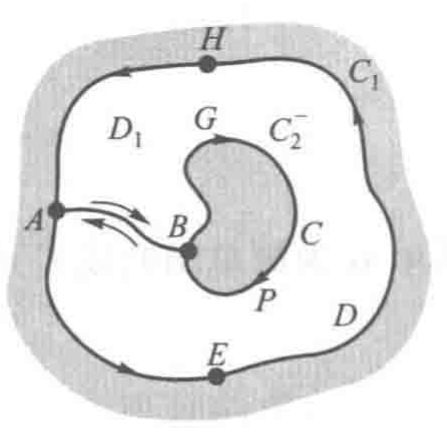
\includegraphics[width=6cm]{闭路变形原理.png}
\end{center}

上式说明,在区域内的一个解析函数沿闭曲线的积分,不因闭曲线在区域内作连续变形而改变它的值。
这一事实称为闭路变形原理。

复合闭路定理:设$C$为多连通区域$D$内的一条简单闭曲线,$C_1,C_2,\cdots,C_n$是在$C$内部的简单闭曲线,
它们互不包含也互不相交,并且以$C,C_1,C_2,\cdots,C_n$为边界的区域全含于$D$,如果$f\left(z\right)$在$D$内解析,则
$$
\oint_Cf\left(z\right)dz=\sum_{k=1}^n\oint_{C_k}f\left(z\right)dz
$$
记$\Gamma$为由$C$及$C_k^-\left(k=1,2,\cdots,n\right)$所组成的复合回路,则
$$
\oint_\Gamma f\left(z\right)dz=0
$$

\begin{center}
    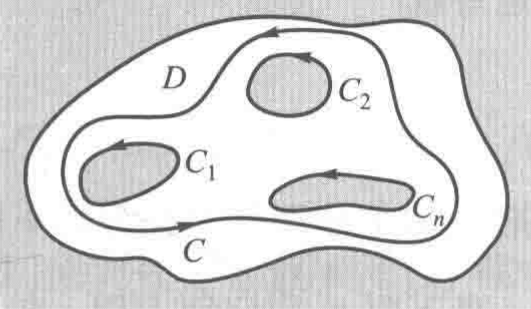
\includegraphics[width=10cm]{复合闭路定理.png}
\end{center}

\subsection{使用原函数积分}

\noindent
\textbf{积分与路径无关}

设函数$f\left(z\right)$在单连通区域$D$内解析,$z_0$与$z_1$为$D$内任意两点,
$C_1$与$C_2$为连接$z_0$与$z_1$的积分路线,且$C_1$与$C_2$都含于$D$,则
$$
\int_{C_1}f\left(z\right)dz=\int_{C_2}f\left(z\right)dz
$$
此时任取$D$内从$z_0$到$z_1$的简单曲线$C$,则积分$\int_Cf\left(z\right)dz$
只与$C$的起点$z_0$和终点$z_1$有关,而与$C$的路径无关,这种积分可以写成
$$
\int_{z_0}^{z_1}f\left(z\right)dz
$$
并把$z_0$和$z_1$分别称为积分的下限和上限。

\noindent
\textbf{原函数}

设在单连通区域$D$内,函数$F\left(z\right)$恒满足条件$F'\left(z\right)=f\left(z\right)$,
则称$F\left(z\right)$是$f\left(z\right)$的原函数。
若$F\left(z\right)$是$f\left(z\right)$的原函数,则对于任意复常数$C$,
$F\left(z\right)+C$也是$f\left(z\right)$的原函数。

设$f\left(z\right)$在单连通区域$D$内解析,且$F\left(z\right)$为$f\left(z\right)$的一个原函数,则
$$
\int_{z_0}^{z_1}f\left(z\right)dz=F\left(z_1\right)-F\left(z_0\right)
$$
其中$z_0$与$z_1$均为区域$D$内的点。

\subsection{柯西积分公式及其推论}

\noindent
\textbf{柯西积分公式}

设$f\left(z\right)$在简单闭曲线$C$所围成的区域$D$内解析,在$\overline{D}=D\cup C$上连续,
$z_0$是$D$内任意一点,则
$$
f\left(z_0\right)=\frac1{2\pi i}\oint_C\frac{f\left(z\right)}{z-z_0}dz
$$

把$z_0$当作变数看待,则可以写成
$$
f\left(z\right)=\frac1{2\pi i}\oint_C\frac{f\left(\zeta\right)}{\zeta-z}d\zeta
$$

\noindent
\textbf{在多连通域内的柯西积分公式}

设$f\left(z\right)$在由简单闭曲线$C_1,C_2$所围成的多连通区域$D$内解析,
在$\overline{D}=C_1+C_2+D$上连续,$C_2$在$C_1$的内部,$z_0$是$D$内任意一点,则
$$
f\left(z_0\right)=\frac1{2\pi i}\oint_{C_1}\frac{f\left(z\right)}{z-z_0}dz
-\frac1{2\pi i}\oint_{C_2}\frac{f\left(z\right)}{z-z_0}dz
$$

\noindent
\textbf{平均值公式}

设$f\left(z\right)$在$\left|z-z_0\right|<R$内解析,在$\left|z-z_0\right|\le R$内连续,则
$$
f\left(z_0\right)=\frac1{2\pi}\int_0^{2\pi}f\left(z_0+Re^{i\theta}\right)d\theta
$$

\noindent
\textbf{最大模原理与最小模原理}

设函数$f\left(z\right)$在区域$D$内解析,又$f\left(z\right)$不是常数,
则$\left|f\left(z\right)\right|$在$D$内没有最大值。

设函数$f\left(z\right)$在区域$D$内解析,且恒不为零,又$f\left(z\right)$不是常数,
则$\left|f\left(z\right)\right|$在$D$内没有最小值。

\subsection{解析函数的高阶导数}

\noindent
\textbf{$n$阶导数公式}

设函数$f\left(z\right)$在简单闭曲线$C$所围成的区域$D$内解析,而在$\overline{D}=D\cup C$上连续,
则$f\left(z\right)$的各阶导数均在$D$内解析,对$D$内任意一点$z$,有
$$
f^{\left(n\right)}\left(z\right)=\frac{n!}{2\pi i}\oint_C
\frac{f\left(\zeta\right)}{\left(\zeta-z\right)^{n+1}}d\zeta
\kern 12pt \left(n\in\mathbb{N}_+\right)
$$

\noindent
\textbf{柯西不等式}

设函数$f\left(z\right)$在$\left|z-z_0\right|<R$内解析,又$\left|f\left(z\right)\right|\le M$
在$\left|z-z_0\right|<R$内恒成立,则
$$
\left|f^{\left(n\right)}\left(z\right)\right|\le \frac{n!M}{R^n}\kern 12pt \left(n\in\mathbb{N}_+\right)
$$

\noindent
\textbf{刘维尔定理}

设函数$f\left(z\right)$在全平面上为解析且有界,则$f\left(z\right)$为一常数。

\subsection{利用留数计算复积分}

\noindent
\textbf{留数的定义与闭合环路积分的关系}

若函数$f\left(z\right)$在$z_0$的某一去心邻域内解析,则
$$
\text{Res}\left[f\left(z\right),z_0\right]=\frac1{2\pi i}\oint_Cf\left(z\right)dz
$$
其中$C$为$z_0$的上述去心邻域内环绕$z_0$的简单闭曲线。

类似的,设$\infty$为$f\left(z\right)$的一个孤立奇点,
即$f\left(z\right)$在圆环域$R<\left|z\right|<+\infty$内解析,则
$$
\text{Res}\left[f\left(z\right),\infty\right]=\frac1{2\pi i}\oint_{C^-}f\left(z\right)dz
\kern 12pt \left(C:\left|z\right|=\rho>R\right)
$$

\noindent
\textbf{留数定理}

设函数$f\left(z\right)$在区域$D$内除有限个孤立奇点$z_1,z_2,\cdots,z_n$外处处解析,
$C$是$D$内包围各奇点的一条正向简单闭曲线,则
$$
\oint_Cf\left(z\right)dz=2\pi i\sum_{k=1}^n\text{Res}\left[f\left(z\right),z_k\right]
$$

\subsection{利用留数计算实积分}

\noindent
\textbf{情形1:形如$\int_0^{2\pi}R\left(\cos\theta,\sin\theta\right)d\theta$的积分}

令$z=e^{i\theta}$,$dz=ie^{i\theta}d\theta$则
$$
\sin\theta=\frac{e^{i\theta}-e^{-i\theta}}{2i}=\frac{z^2-1}{2iz},\kern 12pt
\cos\theta=\frac{e^{i\theta}+e^{-i\theta}}{2}=\frac{z^2+1}{2z}
$$
此时
$$
R\left(\cos\theta,\sin\theta\right)d\theta=
R\left(\frac{z^2-1}{2iz},\frac{z^2+1}{2z}\right)\frac{dz}{iz}
$$
当$\theta$经历变程$\left[0,2\pi\right]$时,对应的$z$正好沿单位圆$\left|z\right|=1$的正向绕行一周。记
$$
f\left(z\right)=R\left(\frac{z^2-1}{2iz},\frac{z^2+1}{2z}\right)\frac1{iz}
$$
$f\left(z\right)$在积分闭路$\left|z\right|=1$上无奇点,在$\left|z\right|<1$内
有$n$个奇点$z_1,z_2,\cdots,z_n$,则
$$
\int_0^{2\pi}R\left(\cos\theta,\sin\theta\right)d\theta=
\oint_{\left|z\right|=1}f\left(z\right)dz=
2\pi i\sum_{k=1}^n\text{Res}\left[f\left(z\right),z_k\right]
$$

\noindent
\textbf{情形2:形如$\int_{-\infty}^{+\infty}R\left(x\right)dx$的积分}

令
$$
R\left(z\right)=\frac{P\left(z\right)}{Q\left(z\right)}=
\frac{a_0z^n+a_1z^{n-1}+\cdots+a_n}{b_0z^m+b_1z^{m-1}+\cdots+b_m}
\kern 12pt \left(a_0b_0\ne0,m-n\ge2\right)
$$
其中$Q\left(z\right)$在实轴上无零点,记$R\left(z\right)$在上半平面$\text{Im}\ z>0$内的极点为
$z_1,z_2,\cdots,z_n$,则
$$
\int_{-\infty}^{+\infty}R\left(x\right)dx=2\pi i\sum_{k=1}^n\text{Res}\left[R\left(z\right),z_k\right]
$$
如果$R\left(z\right)$为偶函数,则
$$
\int_0^{+\infty}R\left(x\right)dx=\frac12\int_{-\infty}^{+\infty}R\left(x\right)dx
=\pi i\sum_{k=1}^n\text{Res}\left[R\left(z\right),z_k\right]
$$

附:如果$Q\left(z\right)$只比$P\left(z\right)$高一次,在柯西主值意义下,
可以将$P\left(z\right)$中最高次项分离出来,并形成一个奇函数(或实变函数意义下的中心对称),
其从$-\infty$到$+\infty$的积分值为零。

\noindent
\textbf{情形3:形如$\int_{-\infty}^{+\infty}R\left(x\right)e^{iax}dx\left(a>0\right)$的积分}

当$R\left(x\right)$是真分式且在实轴上无奇点时,记$f\left(z\right)=R\left(z\right)e^{iaz}$,
其在在上半平面$\text{Im}\ z>0$内的极点为$z_1,z_2,\cdots,z_n$则
$$
\int_{-\infty}^{+\infty}R\left(x\right)e^{iax}dx=
2\pi i\sum_{k=1}^n\text{Res}\left[f\left(z\right),z_k\right]
$$

同时可以得到
$$
\int_{-\infty}^{+\infty}R\left(x\right)\cos\left(ax\right)dx=
\text{Re}\left(2\pi i\sum_{k=1}^n\text{Res}\left[f\left(z\right),z_k\right]\right)
$$
$$
\int_{-\infty}^{+\infty}R\left(x\right)\sin\left(ax\right)dx=
\text{Im}\left(2\pi i\sum_{k=1}^n\text{Res}\left[f\left(z\right),z_k\right]\right)
$$

\noindent
\textbf{附:情形2、3在实轴上有有限个简单极点的情况}

若$R\left(z\right)$在实轴上只有有限个简单极点,可以将这些简单极点的留数值的一半计入求和。
此方法可以通过以下引理证明:

取充分小的$r$,设$f\left(z\right)$沿圆弧
$C_r:z-z_0=re^{i\theta}\left(\theta_1\le\theta\le\theta_2\right)$
上连续,且
$$
\lim_{r\to0}\left(z-z_0\right)f\left(z\right)=\lambda
$$
于$C_r$上一致成立,则有
$$
\lim_{r\to0}\int_{C_r}f\left(z\right)dz=i\left(\theta_2-\theta_1\right)\lambda
$$

\end{document}